The third scenario is based on the second one, (C2), and it tests the appearance of two additional components on two unexpected locations. The birth intensity is defined by the same relation as in Equations \ref{eq:c2-birth} and \ref{eq:c2-birth-means}. The initial states of objects, including the time of birth is also the same and given by Equation \ref{eq:c2-init-states}. However, there are also two additional objects entering the scene at time $k=20$ and $k=60$. Their initial state vector are given by:

\begin{equation}\label{eq:c3-additional-states}
    \svecat{x}{20}{(7)} = \begin{bmatrix}
        -1000.0 \\
        -1000.0 \\
        20.0 \\
        20.0
    \end{bmatrix},
    \qquad
    \svecat{x}{60}{(8)} = \begin{bmatrix}
        1000.0 \\
        1000.0 \\
        -20.0 \\
        -20.0
    \end{bmatrix}.
\end{equation}

The lifespan of these objects is $40$ time steps of each. The whole picture of tracks in the scene is depicted in Figure \ref{fig:c3-scenario}.

\begin{figure*}
    \centering
    \begin{subfigure}[]{0.48\linewidth}
        \centering
        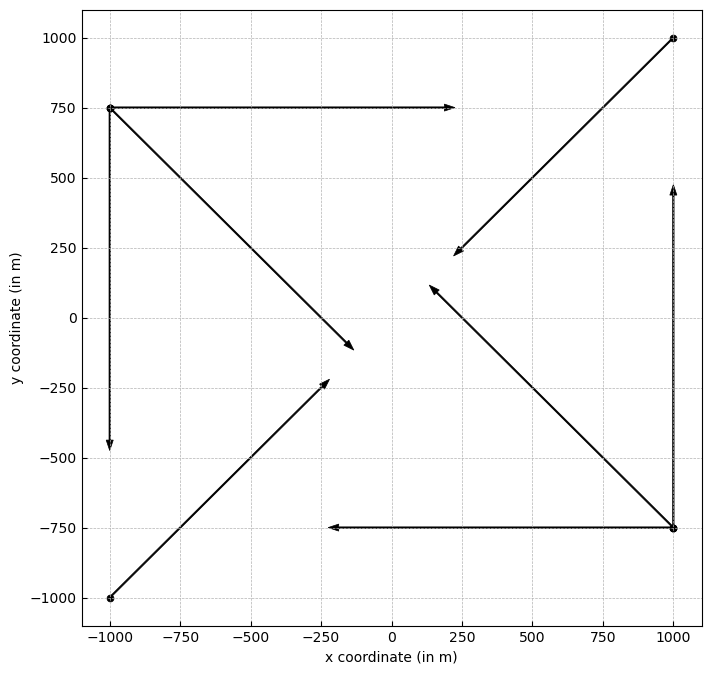
\includegraphics[width=\linewidth]{figures/c3-tracks.png}
    \end{subfigure}
    \hfill
    \begin{subfigure}[]{0.48\linewidth}
        \centering
        \begin{subfigure}[t]{\linewidth}
            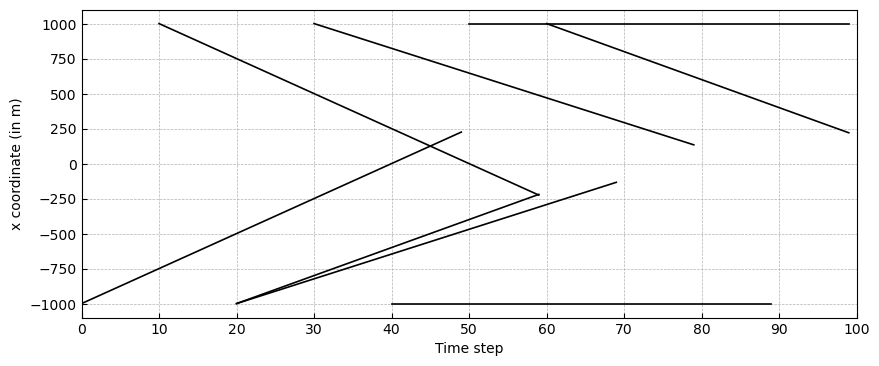
\includegraphics[width=\linewidth]{figures/c3-coord-x.png}
        \end{subfigure}
        \vfill\par
        \begin{subfigure}[b]{\linewidth}
            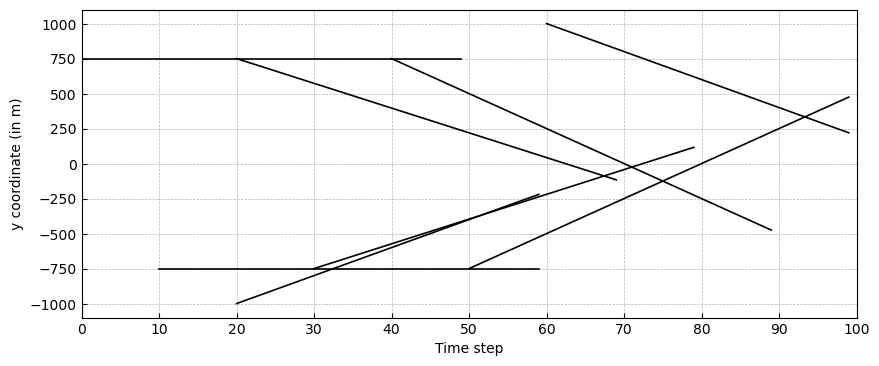
\includegraphics[width=\linewidth]{figures/c3-coord-y.png}
        \end{subfigure}
    \end{subfigure}
  \caption[True tracks of objects in the (C3) and (C4) scenarios.]{The (C3) scenario. In the left figure, we can see the tracks of multiple objects in the 2D space, their locations of birth (black circles) and death (arrow heads). In comparison to the (C2) case, two additional objects appear on two additional positions. The right figure shows how the coordinates of each object track change over time.}
  \label{fig:c3-scenario}
\end{figure*}

For instance, this scenario may occur in cases when a sensor has a blind zone, and the objects appear in the field of view too late. We will later show that without imputation of external information, the GM-PHD filter is unable to capture the dynamics of these objects.
